\documentclass{article}
\usepackage[utf8]{inputenc}
\usepackage[margin = 0.8in]{geometry}
\usepackage{graphicx}
\usepackage{amsmath, amssymb}
\usepackage{subcaption}
\usepackage{multirow}
\usepackage{mathtools}
\usepackage{float}

\title{RBE595 - Week 10 Assignment}
\author{Keith Chester}
\date{Due date: March 21, 2023}

\begin{document}
\maketitle

In this assignment we were tasked with recreating the Figure 8.2 in the text book, which is derived from Example 8.1. Within this, we created a tabular DynaQ agent and tested, for up to 50 episodes each, the agents ability to figure out steps from start to goal with planning steps of 0, 5, and 50 steps allowed.

Below are two charts demonstrating this. The first is all 50 episodes, where as the second we excluded the first two episodes due to the large swing.

\begin{figure}
    \centering
    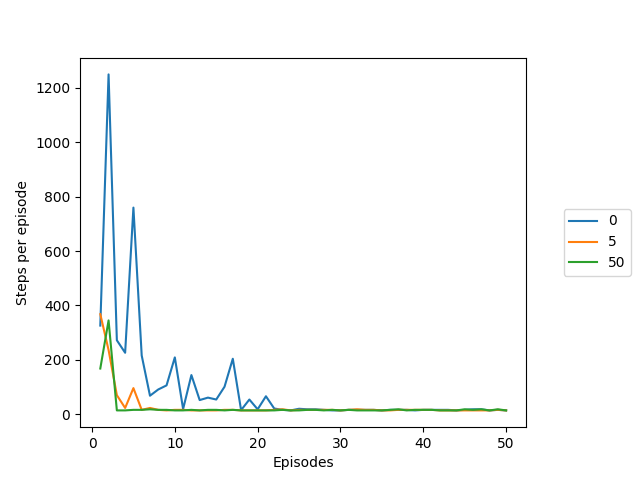
\includegraphics[width=.95\linewidth]{imgs/steps_episodes_full.png}
    \caption{Figure 8.2 Recreated w/ all episodes}
\end{figure}

\begin{figure}
    \centering
    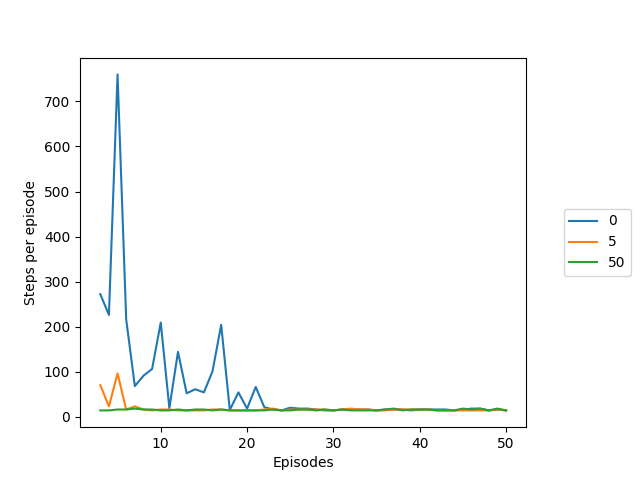
\includegraphics[width=.95\linewidth]{imgs/steps_episodes_sans_episode_2.png}
    \caption{Figure 8.2 Recreated sans the first 2 episodes}
\end{figure}



\end{document}